% !TEX root = Report.tex

\chapter{Summary of \FADBADpp}\label{ch:summary}

We give a brief introduction to \FADBADpp in \SCref{introfadbad}. In \SCref{fadbad}, we introduce the static elementary functions and explain why it is necessary to specialize the struct and overload those functions for a user-defined data type. In \SCref{fadbadforwardmode}, we introduce the mechanism of the implementation of the forward mode in the FADBAD++ package and give a short example to explain how to use that template class. In \SCref{fadbadtaylormode}, we introduce the mechanism of the implementation of the Taylor mode in the FADBAD++ package and give a short example as well.

%\TGN{My scribbles above illustrate how to use the referencing macros. Need elaborate and rewrite. Also, write one such paragraph at the beginning of each chapter except the first.}

\section{Introduction}\label{sc:introfadbad}
The \FADBADpp package contains templates for performing automatic differentiation on functions implemented in C++ code. If the source code of a program, which is an implementation of a differentiable function, is available, then \FADBADpp can be applied to obtain the derivatives of this function \cite{FADBAD++}.

To apply automatic differentiation in a program, the arithmetic type used in the program  is changed to a customized type (\Fn, \B or \T). \F is the template class for the forward mode implementation, \B is the template class for the backward mode implementation, and \T is the template class for the Taylor mode implementation in the \FADBADpp package. 

\section{The fadbad.h file}\label{sc:fadbad}
The file \fadbad implements for a C++ typename {\tt T} a templated struct \Op that contains 29 static member functions. We call these 29 static member functions elementary functions in the following context.

We can call these functions outside the struct \Op to execute arithmetic operations for variables in C++ built-in types, such as float and double.
For example, {\tt Op<double>::myCadd(x,y)} executes {\tt x+=y} for a double type variable {\tt x} and a double type variable {\tt y}.

If {\tt T} is a built-in type, then all the elementary functions in \Op, such as {\tt mySin},  {\tt myCos}, and {\tt myExp}, call their corresponding functions {\tt sin},  {\tt cos}, and {\tt exp} in the C numerics library {\tt math.h}, which only supports C++ built-in types. 
For example, {\tt Op::mySin} is defined by

\texttt{static T mySin(const T \&x) \{ return ::sin(x); \}}

\noindent If {\tt x} is of type float or double, then {\tt Op<T>::mySin(x)}
%, defined by
%\texttt{static T mySin(const T \&x) \{ return ::sin(x); \}} \noindent in the struct \Op,
is equivalent to {\tt sin(x)}, where {\tt sin} is implemented in {\tt math.h}.

However, if {\tt T} is a user-defined data type, say {\tt Interval}, and an elementary function, like {\tt Op<Interval>::myExp}, is not specialized for {\tt Interval}, then it will go to the general template class \Op, and call the function {\tt Op<T>::myExp} inside. But, we cannot simply call {\tt Op<Interval>::myExp(x)} for a {\tt Interval} type variable {\tt x} because the corresponding arithmetic function {\tt exp} defined in {\tt math.h} does not support the type Interval. Similarly, since {\tt Op<Interval>::myExp} is called in the function {\tt fadbad::exp} for a data type {\tt F<Interval>} in the forward mode, as a chain effect, we cannot simply call {\tt fadbad::exp(xf)}, where xf is an {\tt F<Interval>} variable. In Chapter \CHref{extension}, we show how to specialize with the data type \mpreal to the general template class \Op. 

To inform the user about such specializations, \fadbad puts before the templated struct \Op the following message:

{\em The following template allows the user to change the operations that are used in \FADBADpp for computing the derivatives. This is useful as an example for specializing with non-standard types such as interval arithmetic types.}


\section{Forward Method}\label{sc:fadbadforwardmode}
The forward method of AD is implemented by a template class \Fn. An \F object contains a private member m\_val of \U type to store the value and an array of \U type to store the gradient of the variable. Following the chain rule repeatedly, the gradient array inside the result \F object will contain all the partial derivatives with respect to independent variables in the function.

There are two different versions of the \F template class. The version where the gradient array is allocated statically is called stack version, while the other one where the gradient array is allocated dynamically is called heap version. Since the mechanism and usage of these two versions are identical, we will just take the heap version for instance in this report.
\subsection{Overloaded elementary functions in \textbf\texttt{fadiff.h}}
The arithmetic operators and the elementary functions are overloaded in \fadiff. Here, as an example, we give the definition of the overloaded \texttt{sin} function.

%\TGN{This function looks overwhelming. Perhaps give the introductory example first, and then explain how this {\tt sin} works.}

\begin{lstlisting}[numbers=none]
template <typename T>
F<T> sin(const F<T>& a)
{
   F<T> c(Op<T>::mySin(a.val()));
   if (!a.depend())
   return c;
   T tmp(Op<T>::myCos(a.val()));
   c.setDepend(a);
   for (unsigned int i = 0; i < c.size(); ++i)
   c[ i ]            = a[ i ] * tmp;
   return c;
}
\end{lstlisting}

An \F object contains a value and a gradient. In those overloaded functions in \fadiff, the elementary operation functions such as \texttt{mySin},  \texttt{myCos}, and \texttt{myExp} in the \fadbad are called. For example, in the definition of the \texttt{sin} function above, static functions \texttt{mySin} and \texttt{myCos} are called to compute the value and the gradient array. Hence, by following the chain rule step by step, it will output a final result, an \F object with a value and a gradient of \U type inside \cite{IntroAD}. From the gradient array, all the partial derivatives could be obtained with respect to different variables.

\subsection{An introductory example of using the forward mode template class}
Suppose we have the function
\begin{equation}
f(x,y,z)=x+y\times\sin(z)
\label{eq:1}
\end{equation}
Then, we want to obtain partial derivatives with respect to $x$, $y$, and $z$, $df/dx$, $df/dy$, and $df/dz$. Now we are ready to differentiate this function by using the forward method template class \Fn.

If we work with doubles, all the input arguments should be of type \texttt{F<double>} as well as the returned variable.
\begin{lstlisting}[numbers=none]
F<double> func(const F<double>& x, const F<double>& y,  const F<double>& z)
{
	return x+y*sin(z);
}
\end{lstlisting}
Our function above is now prepared for computing derivatives. Before we call the function, we have to specify the variables we want to differentiate with respect to.  After the call, we obtain the function value and the derivatives stored in the object f. This can be done with the following code
\begin{lstlisting}[numbers=none]
F<double> x,y,z,f;   // Declare variables x,y,z,f
x=1;                 // Initialize variable x with value 1
x.diff(0,3);         // Set x as an independent variable of index 0 of 3
y=2;                 // Initialize variable y with value 2
y.diff(1,3);         // Set y as an independent variable of index 1 of 3
z=3;                 // Initialize variable z with value 3
z.diff(2,3);         //	Set z as an independent variable of index 2 of 3
f=func(x,y,z);       // Evaluate function and derivatives
double fval=f.x();   // Value of function
double dfdx=f.d(0);  // Value of df/dx (index 0 of 3)
double dfdy=f.d(1);  // Value of df/dy (index 1 of 3)
double dfdz=f.d(2);  // Value of df/dz (index 2 of 3)
\end{lstlisting}
The forward method is very natural and easy to implement as the flow of derivative information coincides with the order of evaluation \cite{wikiAD}. Suppose we want to compute derivatives with respect to $x$, $y$, and $z$ in the equation \ref{eq:1}. If we apply the chain rule in the forward mode, here are the steps.

\begin{table}[H]
\begin{center}
\begin{tabular}{rl@{\hspace{8mm}}l@{\hspace{8mm}}l}
\hline
\mc{2}{c}{code list} & expression & \mc1c{gradient}  \\\hline
%$v_1$ & $=x$ &  $x$ &$\nabla v_1=(1,0,0) $\\
%$v_2$ & $=y$ &  $y$ &$\nabla v_2=(0,1,0)$\\
%$v_3$ & $=z$  &  $z$ &$\nabla v_3=(0,0,1)$\\
%$v_4$ & $=\sin(v_3)$ & $\sin(z)$&$\nabla v_4=\cos(v_3)\cdot\nabla v_3$\\
%$v_5$ & $=v_2\times v_4$ & $y\sin(z)$&$\nabla v_5=v_2\cdot\nabla v_4 + v_4\cdot\nabla v_2$\\
%$f=v_6$ & $=v_1+ v_5$ & $x+y\sin(z)$&$\nabla v_6=\nabla v_1 + \nabla v_5$\\\hline
&&  $x$ &$\nabla x=(1,0,0) $\\
&&  $y$ &$\nabla y=(0,1,0)$\\
&&  $z$ &$\nabla z=(0,0,1)$\\
$v_1$ & $=\sin(z)$ & $\sin(z)$&$\nabla v_1=\cos(z)\cdot\nabla z$\\
$v_2$ & $=y\times v_1$ & $y\sin(z)$&$\nabla v_2=y\cdot\nabla v_1 + v_1\cdot\nabla y$\\
$f=v_3$ & $=x+ v_2$ & $x+y\sin(z)$&$\nabla v_3=\nabla x + \nabla v_2$\\\hline
\end{tabular}
\end{center}\caption{\label{tb:codelist}Steps of the chain rule in the Forward mode}
\end{table}
Correspondingly, we apply the chain rule to our corresponding function in C++, where the variables $f$, $x$, $y$ and $z$ are of \texttt{F<double>} type. In each step, we represent the temporary result with $v$ of \texttt{F<double>} type comprising the value and the gradient array. 

Here, we explain how to compute the gradients.
\begin{itemize}
	\item First, using \texttt{x.diff(0,3), y.diff(1,3), z.diff(2,3)}, we set independent variables and now $\nabla x=(1,0,0)$, $\nabla y=(0,1,0)$, $\nabla z=(0,0,1)$.
	\item We call the function \texttt{sin} defined in \fadiff to compute the returned variable (denoted as $v_1$) of \texttt{F<double>} type. $v_1$ comprises a value and a gradient array of type double, which are obtained by using the value and gradient array stored in the object z.
	\item Here we evaluate $y \times v1$. The program calls the overloaded operator ``{\tt *}'' in \fadiff and returns a temporary {\tt F<double>} variable denoted as $v_2$. $v_2$ comprises a value and a gradient array of type double, obtained by using the values and gradient arrays of type double stored in object y and $v_1$.
	\item To evaluate $v_1+v_2$, where $v_1, v_2$ are {\tt F<double>} type variables, the program calls the overloaded operator ``{\tt +}'' in \fadiff and returns a temporary {\tt F<double>} variable, denoted as $v_3$.
	\item Finally, $f=v_3$ is processed. The program calls the overloaded operator ``{\tt =}'' in \fadiff. The value and gradient of type double in the object f to the working precision is obtained (because of using double type, the working precision here is 64-bit).
\end{itemize}

\section{Taylor mode and the mechanism of implementation in tadiff.h}\label{sc:fadbadtaylormode}
Taylor mode is implemented by the template class \Tn defined in the file \tadiff. We can use the template class \T to compute the Taylor series of the result of the function.

The functions in \tadiff like {\tt sin}, {\tt exp} will now "record" a directed acyclic graph (DAG) while computing the function value (which is the 0'th order Taylor-coefficient) \cite{FADBAD++}. This DAG can then be used to find the Taylor coefficients if the order of the Taylor expansion is given \cite{IntroAl}.

To obtain the whole DAG for all kinds of available arithmetic operation, an arithmetic operation is supposed to correspond to an unique class type. For example, if we call {\tt sin(x)}, where x is a variable of type {\tt T<double>}, it will create an object of the corresponding class {\tt TTypeNameSin<U, N>} (\texttt{N} is the highest order of the coefficient in the Taylor series, which is 40 by default), meanwhile the 0'th coefficient of the Taylor series in that object is evaluated. Similarly, if we call {\tt exp(x)}, where x is a variable of type {\tt T<double>}, it will create an object of the corresponding class {\tt TTypeNameEXP<U, N>}, meanwhile the 0'th coefficient of the Taylor series in that object is evaluated.

An unary arithmetic operation, say {\tt sin}, corresponds to a class that has a pointer to the single operand, while a binary arithmetic operation, say {\tt pow}, corresponds to a class that has two pointers to the two operands. 

In each corresponded class, the virtual function {\tt eval} is used to compute the resulting Taylor coefficient to the given order using the Taylor coefficients stored in the operand objects. In that function, relevant operation functions from \Opn are called to obtain result values. For example, in the function {\tt eval} in the class {\tt TTypeNameSin<U, N>} which corresponds to the arithmetic operation {\tt sin}, elementary functions from the templated struct \Op, such as {\tt Op<T>::myCos}, {\tt Op<T>::mySin}, {\tt Op<T>::myCadd}, {\tt Op<T>::myCdiv}, and {\tt Op<T>::myCsub} are called inside.
\section{An introductory example of using \textbf\texttt{the Taylor mode template class}}
Suppose we have the function
\begin{equation}
f(x(t),y(t))=x(t)+\sin(y(t))
\label{eq:2}
\end{equation}
We want to obtain the Taylor coefficients of $f(t)$. Now we are ready to compute the Taylor series $f(t)$ by using the Taylor series template class \Tn.

First, we need to adapt our function \ref{eq:2} to a function in C++. All the input arguments should be of type \texttt{T<double>} as well as the returned variable.
\begin{lstlisting}[numbers=none]
T<double> func(const T<double>& x, const T<double>& y)
{
	return x+sin(y);
}
\end{lstlisting}
Before we call the function above, we have to specify the coefficients of the Taylor series in the input variables x and y.  After the call, we obtain coefficients of the Taylor series stored in the object f. This can be done with the following code
\begin{lstlisting}
T<double> x,y,f;     // Declare variables x,y,f
x=1;                 // Initialize 0'th coefficient of x
x[1]=1;              // Initialize 1'st coefficient of x
x[2]=2;              // Initialize 2'nd coefficient of x
y=2;                 // Initialize 0'th coefficient of y
y[1]=1;              // Initialize 1'st coefficient of y
f=func(x,y);         // Evaluate function and record DAG
double fval=f[0];    // Value of function which is also 0'th coefficiet of f
f.eval(10);          // Evaluate Taylor series f to order 10
// f[0]...f[10] now contains the Taylor-coefficients.
\end{lstlisting}
The recorded DAG for this statement is
\begin{figure}[H]
	\centering
	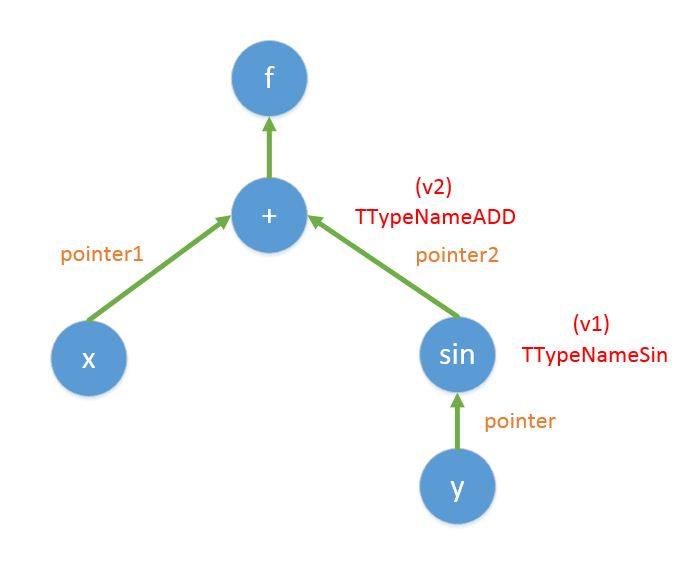
\includegraphics[scale=0.7]{images/DAG1}
	\caption{Directed Acyclic Graph Example}
	%\label{FDD}
\end{figure}
Here are the steps for the AD Taylor mode implementation in the \FADBADpp package.
\begin{itemize}
	\item We initialize x and y of type \texttt{T<double>} and specify the coefficients of the Taylor series for x and y. Thus, the Taylor series of x is $x(t)=1+t+2t^2$ and the Taylor series of y is $y(t)=2+t$.
	\item When processing \texttt{sin(y)}, an object of \texttt{TTypeNameSin<U, N>} type (denoted as $v_1$) will be constructed, which contains a pointer to the single operand y. The 0'th order Taylor-coefficient of v1 will be evaluated.
	\item When we evalute $x+v_1$, an object of \texttt{TTypeNameADD<U, N>} type (denoted as $v_2$) will be constructed, which contains two pointers to operands x and $v_1$ ($v_1$ is of type \texttt{TTypeNameSin<U, N>}). The 0'th order Taylor-coefficient of $v_2$ will be evaluated.
	\item Finally, the result is assigned to variable f. The program calls the overloaded operator ``{\tt =}'' in \fadiff.
	\item If more orders of the Taylor coefficients in f are required, each object like $v_1$ and $v_2$ on the path in the recorded DAG will be re-evaluated to the given order from bottom to top. In the code above, each object in the recorded DAG is re-evaluated to order 10.
\end{itemize}